\documentclass [letterpaper, 12pt] {article}
\usepackage[margin=1in]{geometry}
\usepackage{graphicx, subcaption, ragged2e}
\usepackage{amsmath}
\usepackage{epsfig}
\usepackage{parskip}
\usepackage[utf8]{inputenc}
\usepackage[english]{babel}
\usepackage{cite}

\begin{document}

	\begin{titlepage}
	\centering
	\vspace*{\fill}

	\vspace*{0.5cm}

	\huge\bfseries
	TITLE GOES HERE
	
	\vspace*{0.5cm}

	\large Luke Mattfeld

	\vspace*{\fill}
	\end{titlepage}

\pagenumbering{roman}
\tableofcontents
\newpage
\pagenumbering{arabic}

\section {Abstract}

here is where one writes the abstract.  Words, words, words, words, words, words.  Words, words, words, words, words, words. Words, words, words, words, words, words. Words, words, words, words, words, words. Words, words, words, words, words, words. Words, words, words, words, words, words. Words, words, words, words, words, words. Words, words, words, words, words, words. Words, words, words, words, words, words. Words, words, words, words, words, words. Words, words, words, words, words, words. Words, words, words, words, words, words. Words, words, words, words, words, words. Words, words, words, words, words, words. Words, words, words, words, words, words.
\pagebreak

\section {Introduction}

The Plague is a dangerous disease that has greatly affected human history in it’s 3 major outbreaks. These outbreaks include the Justinian Plague, the Bubonic Plague, and the more recent outbreak in the 1800’s in China. [citation needed]

This plague, powered by the bacteria known as Yersinia Pestis, has 3 primary strains:
Bubonic, the most well-known, manifests in painful, swollen “Buboes” at or near the lymph nodes, and is spread through contact with insects biting the human skin (Better phrasing needed).
Pneumonic, also fairly deadly, is spread through aspirated bacteria, and starts in the lungs. It is spread through aspiration in the presence of infected individuals or in an environment laiden with the bacteria.
Finally, there is a systemic variant which is the most deadly. It has little in terms of incubation, and spreads fast throughout the body. (Blood vessels pop [citation needed]). This had little effect on the overall epidemic when compared to the Bubonic and Pneumonic strains.
(Mortality rates for each needed)

While the pneumonic and systemic variants did play a role in the epidemic, and in fact the pneumonic plague often followed in a secondary outbreak wave, the spreading of the bubonic plague is the subject of this study.

While historical evidence has provided prolific details as to how the various outbreaks of the Plague have affected society, art, and culture, little is known for sure about the way in which the plague spread. The state of medical technology at the time has led to speculation and deductive reasoning from the available data. From this the currently accepted theory has been formed: The Bubonic plague was mostly spread through the interaction of rat and flea populations. The fleas host the disease contracted through biting a host. The fleas then are carried by the rats, which are not significantly affected by the disease. Once a carrying capacity for the rat has been reached, the flea is forced to find another host. Due to the nature of the bacteria, the digestive tract of the flea is “clogged up” (better alliteration needed) and the flee is pushed to constant biting due to hunger. The flea then regurgitates the bacteria into the many open bites. In this way the bacteria enters the new host. 
Due to the poor hygienic situation in Europe at the time, the presence of rats and fleas in and around human habitation was common. Thus, when infected rats arrived through trade routes and incoming ships, the population was quickly infected. 
This theory is backed somewhat by historical evidence - as sightings of sick rats were observed, and were thought to bring “bad air” which was the source of new infection. [citation needed]

However recent studies looking at the mathematical models underlying this type of disease spread seems to show the widely-held theory of transmission may not be correct. The paper which provided jumping off point for this one investigates fitting the model of the prevailing rat-flea theory and a new model that looks at the interaction of human fleas and lice to the historical death rates. The conclusion was that, given the evidence, the new model better predicted the death curve over the course of the 2nd wave of the disease [citation needed].

(Note: For the citations, I do have them saved. I just need to figure out Latex' References.bib)
\pagebreak

\section {Background}


\pagebreak

\section {Mathematical Modeling}

Do some intro to section.  
Words, words, words, words, words, words.  Words, words, words, words, words, words. Words, words, words, words, words, words. Words, words, words, words, words, words. Words, words, words, words, words, words. Words, words, words, words, words, words. Words, words, words, words, words, words. Words, words, words, words, words, words. Words, words, words, words, words, words. Words, words, words, words, words, words. Words, words, words, words, words, words. Words, words, words, words, words, words. Words, words, words, words, words, words. Words, words, words, words, words, words. Words, words, words, words, words, words. 


\subsection {Pneumonic Plague}

Following these simplified changes in
populations, the system of equations would be as follows:
\begin{align} 
	\frac{dS}{dt}  &=  -\alpha SI \\ 
	\frac{dE}{dt}  &=  \alpha SI - \sigma E \\
	\frac{dI}{dt}  &=  \sigma E - \nu I - rI \\
	\frac{dR}{dt} &= rI
\end{align}

Here ias a figure, however eps files should be used (not jpg nor png flies).
\begin{figure}[h!]
	\begin{subfigure}{0.48\textwidth}
		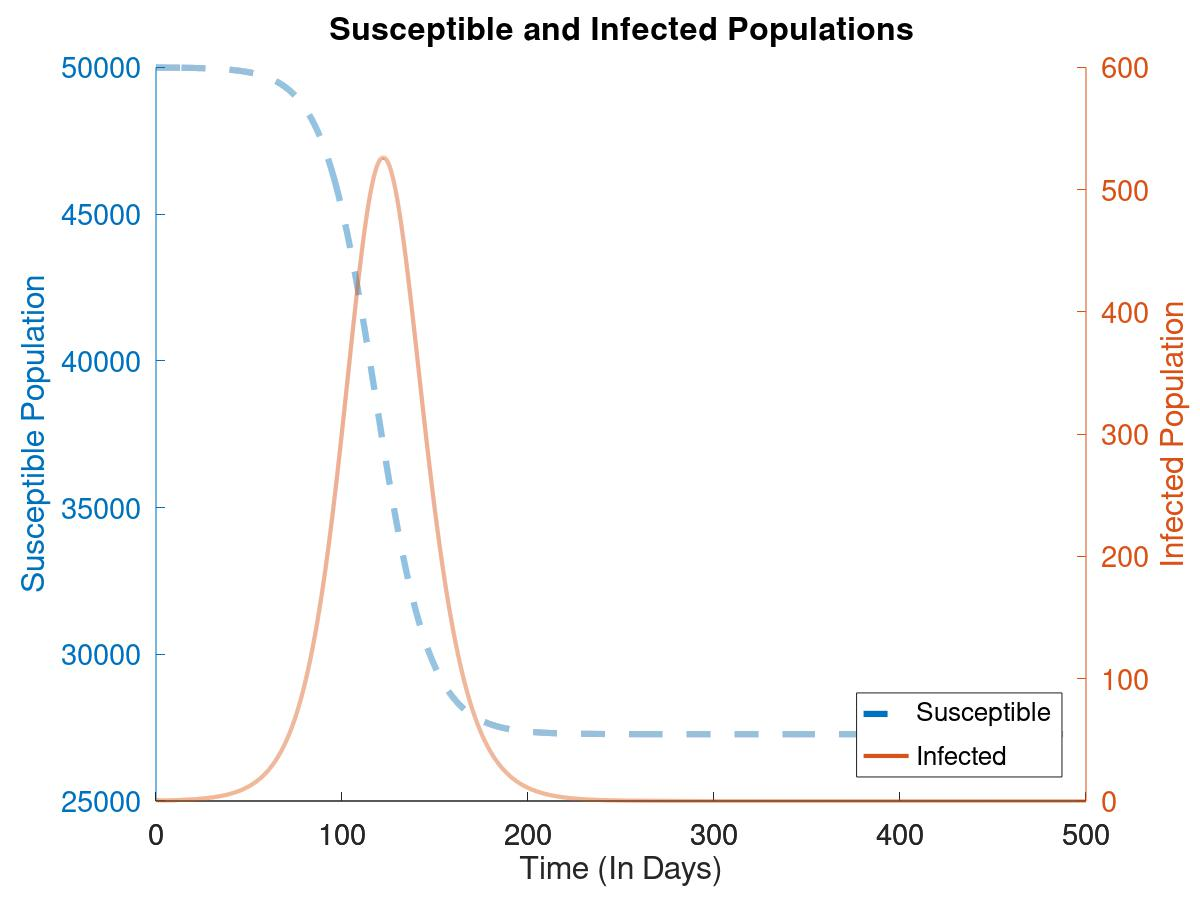
\includegraphics[width=\linewidth]{Figures/short_pneumonic.jpg}
	\end{subfigure}\hspace{\fill}
	\begin{subfigure}{0.48\textwidth}
		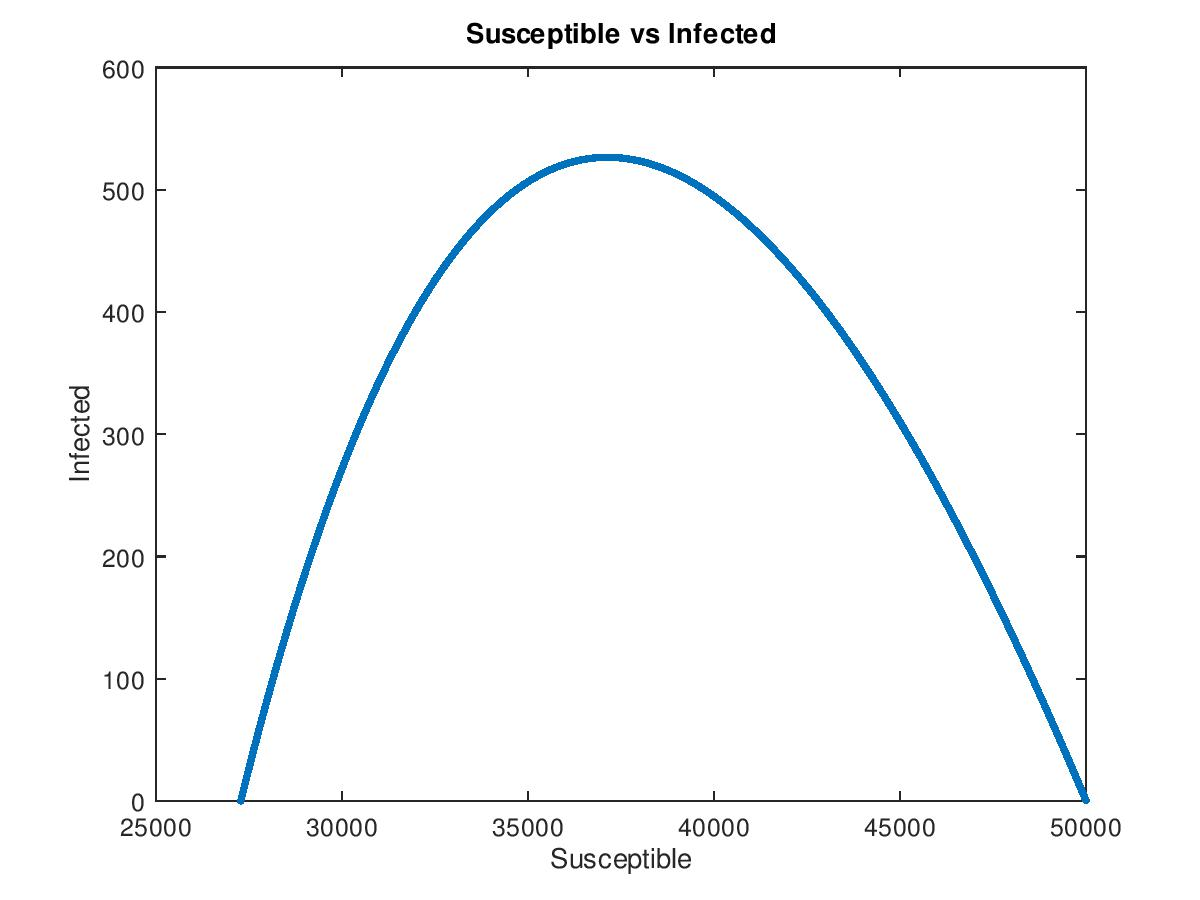
\includegraphics[width=\linewidth]{Figures/short_pneumonic2.jpg}
	\end{subfigure}
	\caption{Pre-treatment susceptible and infected population. $\alpha=2*10^{-5}, \sigma=0.33, \nu=0.75, r=0$.
	The rise and decrease of pneumonic plague victims pre-treatment, leading to a disease free state. The susceptible
	population is plotted against the infected population showing the relationship between the two populations.} 
\end{figure}

From the results 
\pagebreak

\subsubsection{special case}

Examination of this case Words, words, words, words, words, words.  Words, words, words, words, words, words. Words, words, words, words, words, words. Words, words, words, words, words, words. Words, words, words, words, words, words. Words, words, words, words, words, words. Words, words, words, words, words, words. Words, words, words, words, words, words. Words, words, words, words, words, words. Words, words, words, words, words, words. Words, words, words, words, words, words. Words, words, words, words, words, words. Words, words, words, words, words, words. Words, words, words, words, words, words. Words, words, words, words, words, words. 


\pagebreak

\subsubsection{a different case}
Examination of this case Words, words, words, words, words, words.  Words, words, words, words, words, words. Words, words, words, words, words, words. Words, words, words, words, words, words. Words, words, words, words, words, words. Words, words, words, words, words, words. Words, words, words, words, words, words. Words, words, words, words, words, words. Words, words, words, words, words, words. Words, words, words, words, words, words. Words, words, words, words, words, words. Words, words, words, words, words, words. Words, words, words, words, words, words. Words, words, words, words, words, words. Words, words, words, words, words, words. 

\pagebreak

\subsection {Bubonic Plague}

Words, words, words, words, words, words. Words, words, words, words, words, words. Words, words, words, words, words, words. Words, words, words, words, words, words. Words, words, words, words, words, words. Words, words, words, words, words, words. Words, words, words, words, words, words. Words, words, words, words, words, words. Words, words, words, words, words, words. Words, words, words, words, words, words. Words, words, words, words, words, words. Words, words, words, words, words, words. Words, words, words, words, words, words. Words, words, words, words, words, words. 



\subsubsection {Rat and Flea Dynamics}
TWords, words, words, words, words, words. Words, words, words, words, words, words. Words, words, words, words, words, words. Words, words, words, words, words, words. Words, words, words, words, words, words. Words, words, words, words, words, words. Words, words, words, words, words, words. Words, words, words, words, words, words. Words, words, words, words, words, words. Words, words, words, words, words, words. Words, words, words, words, words, words. Words, words, words, words, words, words. Words, words, words, words, words, words. Words, words, words, words, words, words. 


\begin{align}
	\frac{dR_c}{dt} &= \alpha \frac{F_c}{F_T} (R_T-R_c)  - \gamma R_c \\
	\frac{dF_c}{dt} &= \lambda \frac{R_c}{R_T} (F_T-F_c) - \rho F_c 
\end{align}
Words, words, words, words, words, words. Words, words, words, words, words, words. Words, words, words, words, words, words. Words, words, words, words, words, words. Words, words, words, words, words, words. Words, words, words, words, words, words. Words, words, words, words, words, words. Words, words, words, words, words, words. Words, words, words, words, words, words. Words, words, words, words, words, words. Words, words, words, words, words, words. Words, words, words, words, words, words. Words, words, words, words, words, words. Words, words, words, words, words, words. 


This results in a system of the following:

\begin{align}
	\frac{dr}{d\tau} &= Af(1-r)-rG \\
	\frac{df}{d\tau} &= Yr(1-f)-f
\end{align}

Where $A=\frac{\alpha}{\rho}, G=\frac{\gamma}{\rho},
Y=\frac{\lambda}{\rho}$.
The next steps are to find the nullclines of the system and then determine the equilibria, which are
(0, 0) and [$\frac{AY-G}{Y(A+G)}, \frac{AY-G}{A(1+Y)}$]. The nullclines can be found by setting
$\frac{dr}{dt}$ equal to zero and $\frac{df}{dt}$ equal to zero as well and solving for either r or f,
in this case solve for f as this is the flea population.

\begin{align}
	f &= \frac{rG}{A(1-r)} \\
	f &= \frac{rY}{rY+1}
\end{align}

\begin{figure}[h!]
	\begin{subfigure}{0.48\linewidth}
	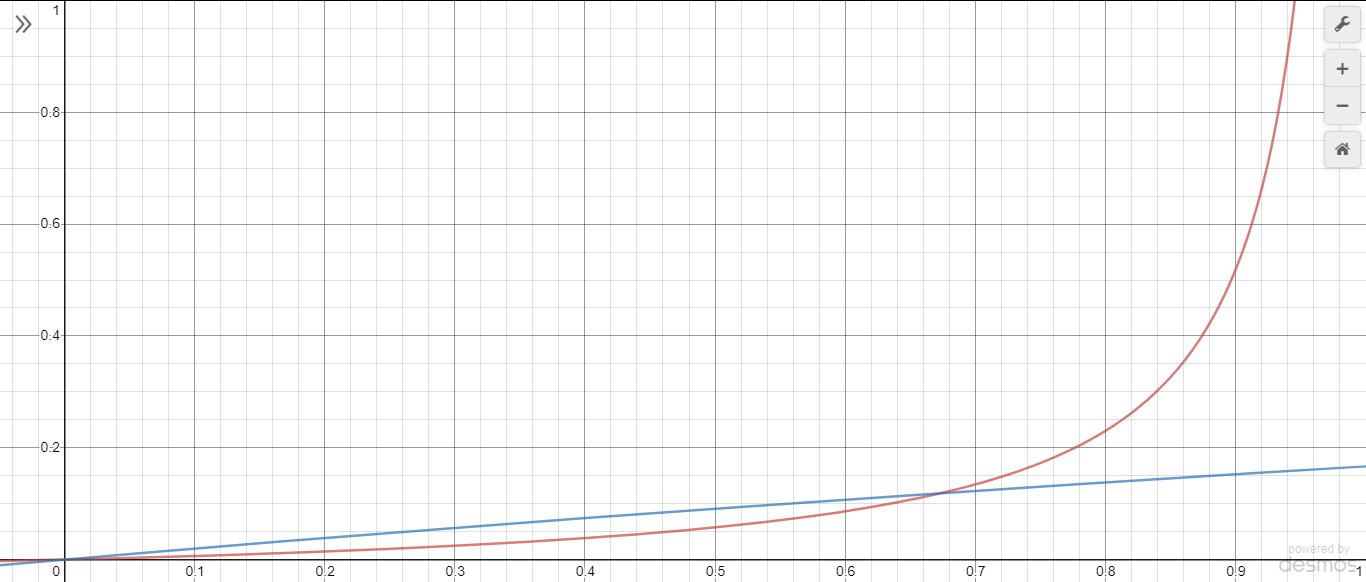
\includegraphics[width=\linewidth]{Figures/Nullcline.png}
	\end{subfigure}
	\begin{subfigure}{0.48\linewidth}
	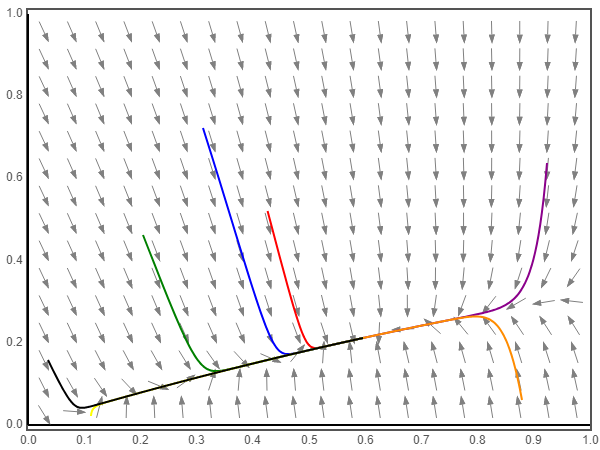
\includegraphics[width=\linewidth]{Figures/nullcline2.png}
	\end{subfigure}
	\caption{Nullclines of the system of rat and flea dynamics and trajectories in phase space.}
\end{figure}

Now comes determining the Jacobian,
a matrix comprised of the partial derivative of each compartment with respect to one variable.
In this case, the Jacobian matrix is given by 
\begin{equation}
J(r, f)=
\begin{bmatrix}
-Af-G & A-Ar \\
Y-Yf & -Yr-1
\end{bmatrix}
\end{equation}

To study the stability of the equilibria, we need to plug in the equilibrium points
into the matrix for their respective variables. When r*=0 and f*=0, the resultant trace
of the Jacobian is going to be $-G-1$, which will always be a negative number seeing as G is a positive number. 
With the trace of the Jacobian being less then zero, there are two
possibilities for the stability of this equilibrium, which will depend on the determinant, being either an
asymptotically stable node or an asymptotically unstable spiral. Studying the determinant of the matrix
under the specified r* and f*, the determinant will be $G-AY$. This means that the stability of the point
will change, if $G<AY$, then the determinant will be negative which results in the point being an unstable
spiral. If $G>AY$, then the determinant will be positive which results in a stable node. When 
r*=$\frac{AY-G}{Y(A+G)}$ and f*=$\frac{AY-G}{A(1+Y)}$ the computations become more
complicated as the computation is algebraically heavy. The Jacobian matrix that results
from these specific values of f and r is
\begin{equation}
J(r*, f*)=
\begin{bmatrix}
-\frac{AY-G}{A+G}-G & A-\frac{A^{2}Y-AG}{Y(A+G)} \\
Y-\frac{AY^{2}-GY}{A(1+Y)} & -\frac{AY-G}{A+G}-1 \\
\end{bmatrix}
\end{equation}
The resulting trace of the Jacobian matrix is $-2(\frac{AY-G}{A+G})-G-1$ which is only positive
provided $2G-2AY>A+G+AG+G^{2}$. Otherwise, the trace is going to be negative. The determinant
of the Jacobian matrix is $$(\frac{AY-G}{A+G})^{2} + (G+1)\frac{AY-G}{A+G}+G-AY+\frac{AY^{2}-GY}{1+Y} + \frac{A^{2}Y-AG}{A+G}-(\frac{A^{2}Y-AG}{Y(A+G)}\frac{AY^{2}-GY}{A(1+Y)})$$
With this determinant and trace, the equilibrium is uncertain as it could be stable or unstable, node or spiral
depending on the parameter estimates of the terms. From examining the history of the disease,
we can assume that the r* and f* equilibrium is being met seeing that the rat and flea
populations continue to spread plague through different areas of the world.

\pagebreak

\subsubsection{Plague Dynamics Coupled with Rat and Flea Dynamics}

Words, words, words, words, words, words. Words, words, words, words, words, words. Words, words, words, words, words, words. Words, words, words, words, words, words. Words, words, words, words, words, words. Words, words, words, words, words, words. Words, words, words, words, words, words. Words, words, words, words, words, words. Words, words, words, words, words, words. Words, words, words, words, words, words. Words, words, words, words, words, words. Words, words, words, words, words, words. Words, words, words, words, words, words. Words, words, words, words, words, words. 


Words, words, words, words, words, words. Words, words, words, words, words, words. Words, words, words, words, words, words. Words, words, words, words, words, words. Words, words, words, words, words, words. Words, words, words, words, words, words. Words, words, words, words, words, words. Words, words, words, words, words, words. Words, words, words, words, words, words. Words, words, words, words, words, words. Words, words, words, words, words, words. Words, words, words, words, words, words. Words, words, words, words, words, words. Words, words, words, words, words, words. 

\begin{align}
	\frac{dR_T}{dt} &= (\frac{\beta_R}{K_R})R_T(K_R-R_T)-\delta R_c \\
	\frac{dR}{dt} &= (\frac{\beta_R}{K_R})R_T(K_R-R)-\alpha \frac{F_c}{F_T}R+\gamma  R_c \\
	\frac{dR_c}{dt} &= \alpha \frac{F_c}{F_T} (R_T-R_c)-\frac{\beta_R}{K_R}(R_T)(R_c) - \delta R_c - \gamma R_c 
\end{align}
Words, words, words, words, words, words. Words, words, words, words, words, words. Words, words, words, words, words, words. Words, words, words, words, words, words. Words, words, words, words, words, words. Words, words, words, words, words, words. Words, words, words, words, words, words. Words, words, words, words, words, words. Words, words, words, words, words, words. Words, words, words, words, words, words. Words, words, words, words, words, words. Words, words, words, words, words, words. Words, words, words, words, words, words. Words, words, words, words, words, words. 


\begin{align}
	\frac{dF_T}{dt} &= (\frac{\beta_F}{K_F})F_T(K_F-F_T)-\rho F_T  \\
	\frac{dF_c}{dt} &= \lambda \frac{R_c}{R_T} (F_T-F_c) - \rho F_c 
\end{align}

Words, words, words, words, words, words. Words, words, words, words, words, words. Words, words, words, words, words, words. Words, words, words, words, words, words. Words, words, words, words, words, words. Words, words, words, words, words, words. Words, words, words, words, words, words. Words, words, words, words, words, words. Words, words, words, words, words, words. Words, words, words, words, words, words. Words, words, words, words, words, words. Words, words, words, words, words, words. Words, words, words, words, words, words. Words, words, words, words, words, words. 



The human dynamics follow an SEIR model where the inflow to the infected state depends on the
population density of the contaminated fleas and an interaction term for the two populations.

\begin{align}
	\frac{dS}{dt} &= \beta (S+R_b) - \sigma S \frac{F_c}{F_T} - \mu S \\
	\frac{dE}{dt} &= \sigma S \frac{F_c}{F_T} - \nu E - \mu E \\
	\frac{dI}{dt} &= \nu E - \phi I - rI \\
	\frac{dR_b}{dt} &= rI - \mu R_b
\end{align}

Words, words, words, words, words, words. Words, words, words, words, words, words. Words, words, words, words, words, words. Words, words, words, words, words, words. Words, words, words, words, words, words. Words, words, words, words, words, words. Words, words, words, words, words, words. Words, words, words, words, words, words. Words, words, words, words, words, words. Words, words, words, words, words, words. Words, words, words, words, words, words. Words, words, words, words, words, words. Words, words, words, words, words, words. Words, words, words, words, words, words. 



In this model, when looking at every part of the model, there are going to be certain parameters
that will be fixed, such as the carrying capacity of fleas in relation to the population of the rats.
Other fixed parameters are the parameters for the birth rate of humans, the intrinsic death rate of
people, the birth and death rates of rats and fleas, the carrying capacity of the rats, incubation period
in humans, death rate, and the recovery rate in both humans and rats.

\begin{figure}[h!]
	\begin{subfigure}{0.48\textwidth}
	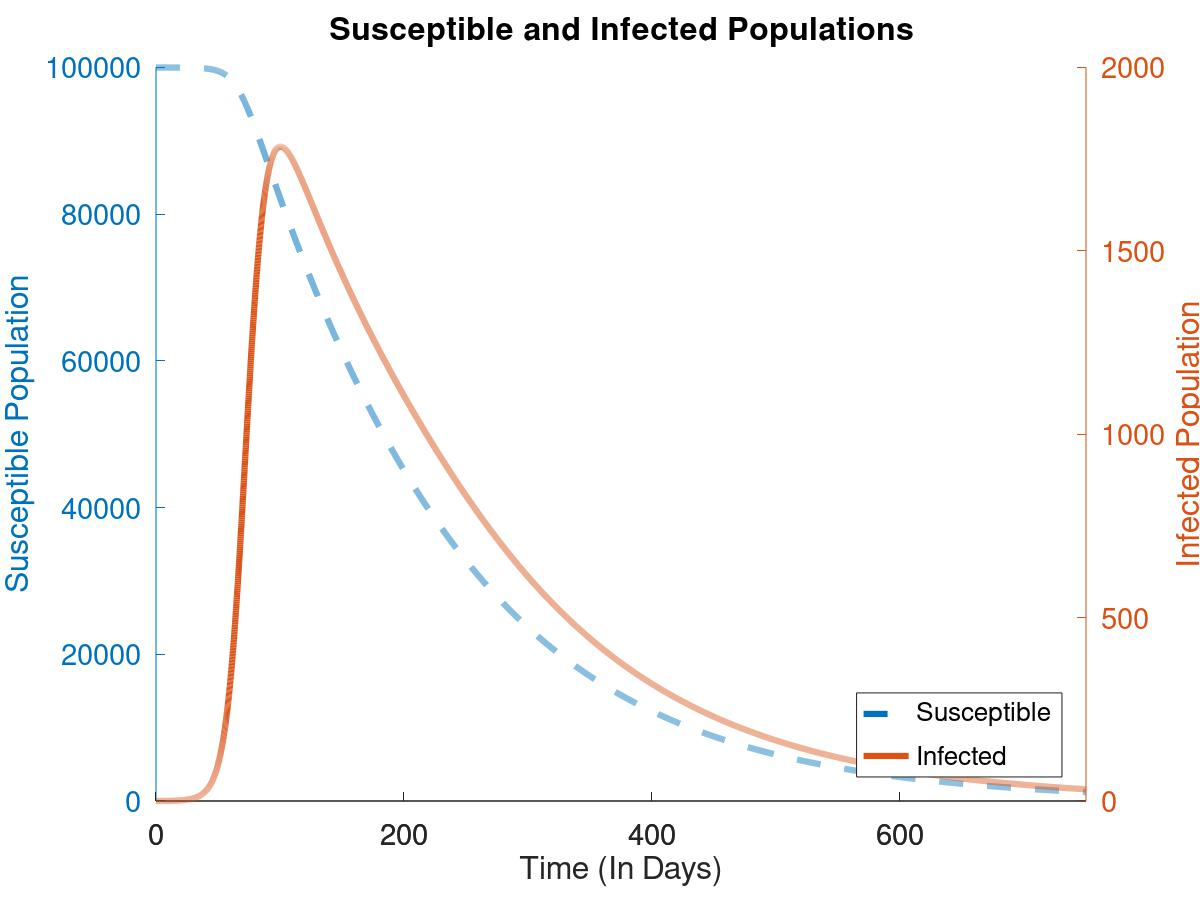
\includegraphics[width=\linewidth]{Figures/bubonic750.jpg}
	\end{subfigure}\hspace{\fill}
	\begin{subfigure}{0.48\textwidth}
	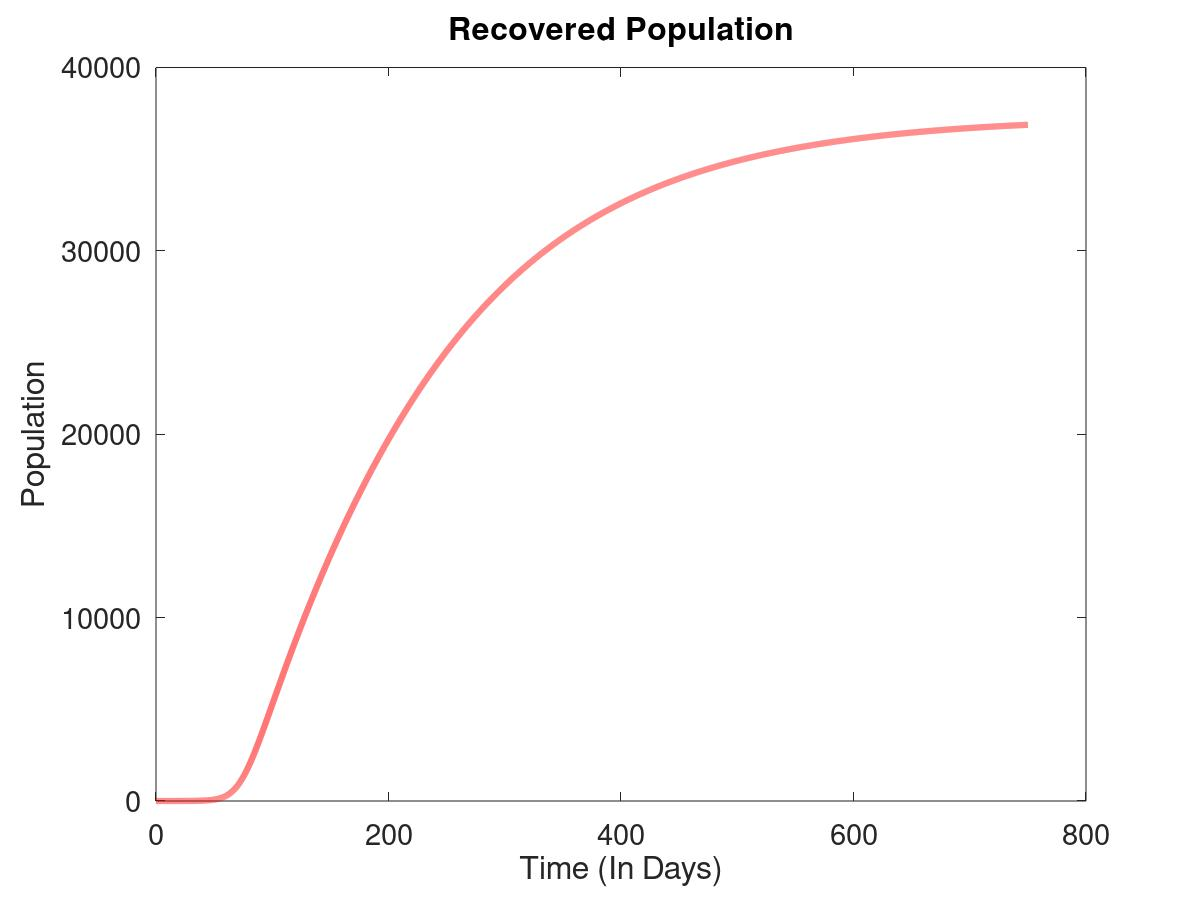
\includegraphics[width=\linewidth]{Figures/bubonicr.jpg}
	\end{subfigure}
	\begin{subfigure}{0.48\textwidth}
	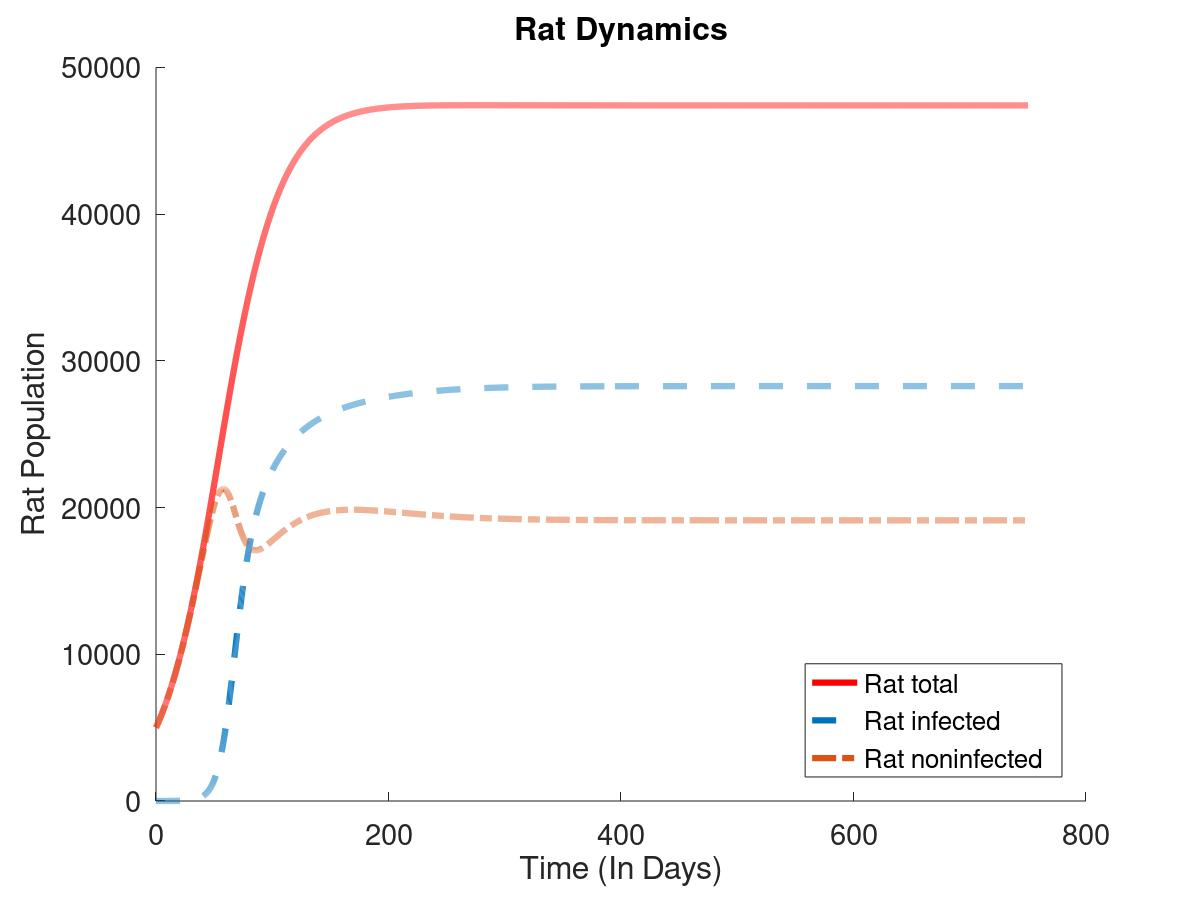
\includegraphics[width=\linewidth]{Figures/bubonicrat.jpg}
	\end{subfigure}\hspace{\fill}
	\begin{subfigure}{0.48\textwidth}
	\includegraphics[width=\linewidth]{Figures/Bubonicrf.jpg}
	\end{subfigure}
	\caption{Human, rat, and flea populations under the bubonic model. The parameters are $\alpha=0.25, \delta=1/300, \gamma=0.1, \lambda=0.2, \rho=1/40, \sigma=1.5*10^{-3}, \nu=1/6, \phi=1/6, r=1/10.$}
\end{figure}

Words, words, words, words, words, words. Words, words, words, words, words, words. Words, words, words, words, words, words. Words, words, words, words, words, words. Words, words, words, words, words, words. Words, words, words, words, words, words. Words, words, words, words, words, words. Words, words, words, words, words, words. Words, words, words, words, words, words. Words, words, words, words, words, words. Words, words, words, words, words, words. Words, words, words, words, words, words. Words, words, words, words, words, words. Words, words, words, words, words, words. 



Words, words, words, words, words, words. Words, words, words, words, words, words. Words, words, words, words, words, words. Words, words, words, words, words, words. Words, words, words, words, words, words. Words, words, words, words, words, words. Words, words, words, words, words, words. Words, words, words, words, words, words. Words, words, words, words, words, words. Words, words, words, words, words, words. Words, words, words, words, words, words. Words, words, words, words, words, words. Words, words, words, words, words, words. Words, words, words, words, words, words. 


\newpage

\section {Discussion}

Words, words, words, words, words, words. Words, words, words, words, words, words. Words, words, words, words, words, words. Words, words, words, words, words, words. Words, words, words, words, words, words. Words, words, words, words, words, words. Words, words, words, words, words, words. Words, words, words, words, words, words. Words, words, words, words, words, words. Words, words, words, words, words, words. Words, words, words, words, words, words. Words, words, words, words, words, words. Words, words, words, words, words, words. Words, words, words, words, words, words. 



Words, words, words, words, words, words. Words, words, words, words, words, words. Words, words, words, words, words, words. Words, words, words, words, words, words. Words, words, words, words, words, words. Words, words, words, words, words, words. Words, words, words, words, words, words. Words, words, words, words, words, words. Words, words, words, words, words, words. Words, words, words, words, words, words. Words, words, words, words, words, words. Words, words, words, words, words, words. Words, words, words, words, words, words. Words, words, words, words, words, words. 




Words, words, words, words, words, words. Words, words, words, words, words, words. Words, words, words, words, words, words. Words, words, words, words, words, words. Words, words, words, words, words, words. Words, words, words, words, words, words. Words, words, words, words, words, words. Words, words, words, words, words, words. Words, words, words, words, words, words. Words, words, words, words, words, words. Words, words, words, words, words, words. Words, words, words, words, words, words. Words, words, words, words, words, words. Words, words, words, words, words, words. 



Words, words, words, words, words, words. Words, words, words, words, words, words. Words, words, words, words, words, words. Words, words, words, words, words, words. Words, words, words, words, words, words. Words, words, words, words, words, words. Words, words, words, words, words, words. Words, words, words, words, words, words. Words, words, words, words, words, words. Words, words, words, words, words, words. Words, words, words, words, words, words. Words, words, words, words, words, words. Words, words, words, words, words, words. Words, words, words, words, words, words. 




\pagebreak

\bibliography{References.bib}
\bibliographystyle{plain}

\end{document}